%%%%%%%%%%%%%%%%%%%%%%%%%%%%%%%%%%%%%%%%%
% University Assignment Title Page 
% LaTeX Template
% Version 1.0 (27/12/12)
%
% This template has been downloaded from:
% http://www.LaTeXTemplates.com
%
% Original author:
% WikiBooks (http://en.wikibooks.org/wiki/LaTeX/Title_Creation)
%
% License:
% CC BY-NC-SA 3.0 (http://creativecommons.org/licenses/by-nc-sa/3.0/)
% 
% Instructions for using this template:
% This title page is capable of being compiled as is. This is not useful for 
% including it in another document. To do this, you have two options: 
%
% 1) Copy/paste everything between \begin{document} and \end{document} 
% starting at \begin{titlepage} and paste this into another LaTeX file where you 
% want your title page.
% OR
% 2) Remove everything outside the \begin{titlepage} and \end{titlepage} and 
% move this file to the same directory as the LaTeX file you wish to add it to. 
% Then add \input{./title_page_1.tex} to your LaTeX file where you want your
% title page.
%
%%%%%%%%%%%%%%%%%%%%%%%%%%%%%%%%%%%%%%%%%
%\title{Title page with logo}
%----------------------------------------------------------------------------------------
%	PACKAGES AND OTHER DOCUMENT CONFIGURATIONS
%----------------------------------------------------------------------------------------

\documentclass[12pt, spanish]{article}
\usepackage[spanish]{babel}
\selectlanguage{spanish}
\usepackage[utf8x]{inputenc}
\usepackage{amsmath}
\usepackage{graphicx}
\usepackage{subcaption}
\usepackage{utopia}
\pagestyle{headings}

\usepackage[colorinlistoftodos]{todonotes}
\usepackage[acronym,automake]{glossaries}
\usepackage{hyperref}
\usepackage[font=small,labelfont=bf]{caption}

\renewcommand{\baselinestretch}{1.5}


\raggedbottom                            %Evita que LaTeX distribuya los espacios en blanco sobre la página, en lugar de eso los envía al fondo

\makeglossaries
\newacronym{GTC}{GTC}{Gran Telescopio de Canarias}
\newacronym{IA-UNAM}{IA-UNAM}{Instituto de Astronom\'ia – Universidad Nacional Aut\'onoma de M\'exico}
\newacronym{PFC}{PFC}{Proyecto Fin de Carrera}
\newacronym{SSL}{SSL}{Secure Socket Layer}
\newacronym{ANSI}{ANSI}{American National Standards Institute}
\newacronym{CNRI}{CNRI}{Corporation for National Research Initiatives}
\newacronym{PSF}{PSF}{Python Software Foundation}
\newacronym{PSFL}{PSFL}{Python Software Foundation Licence}
\newacronym{FSF}{FSF}{Free Software Foundation}
\newacronym{AP}{AP}{Access Point}
\newacronym{NIST}{NIST}{Instituto Nacional de Estándares y Tecnología}
\newacronym{LR-WPAN}{LR-WPAN}{Low-Rate Wireless Personal Area Network}
\newacronym{PAM}{PAM}{Pluggable Authentication Modules}
\newacronym{IDE}{IDE}{Integrated Development Environment}
\newacronym{CA}{CA}{Certificate Authority}
\newacronym{CSR}{CSR}{Certificate Signing Request}


\begin{document}
\begin{titlepage}

\newcommand{\HRule}{\rule{\linewidth}{0.5mm}} % Defines a new command for the horizontal lines, change thickness here

\center % Center everything on the page
 
%----------------------------------------------------------------------------------------
%	HEADING SECTIONS
%----------------------------------------------------------------------------------------

\textsc{\LARGE Shidix Technologies}\\[1.5cm] % Name of your university/college
\textsc{\Large Calculadora de tiempos de exposici\'on}\\[0.5cm] % Major heading such as course name
\textsc{\large Especificaciones}\\[0.5cm] % Minor heading such as course title

%----------------------------------------------------------------------------------------
%	TITLE SECTION
%----------------------------------------------------------------------------------------

\HRule \\[0.4cm]
{ \huge \bfseries FRIDA}\\[0.4cm] % Title of your document
\HRule \\[1.5cm]
 
%----------------------------------------------------------------------------------------
%	AUTHOR SECTION
%----------------------------------------------------------------------------------------

\begin{minipage}{0.4\textwidth}
\begin{flushleft} \large
\emph{Preparado por:}\\
Daniel Jacobo D\'iaz Gonz\'alez
\end{flushleft}
\end{minipage}
~
\begin{minipage}{0.4\textwidth}
\begin{flushright} \large
\emph{Aprobado por:} \\
Jos\'e Acosta
\end{flushright}
\end{minipage}\\[2cm]

% If you don't want a supervisor, uncomment the two lines below and remove the subsection above
%\Large \emph{Author:}\\
%John \textsc{Smith}\\[3cm] % Your name

%----------------------------------------------------------------------------------------
%	DATE SECTION
%----------------------------------------------------------------------------------------

{\large \today}\\[2cm] % Date, change the \today to a set date if you want to be precise

%----------------------------------------------------------------------------------------
%	LOGO SECTION
%----------------------------------------------------------------------------------------

\begin{figure*}[h]
    \centering
    \begin{subfigure}[b]{0.5\textwidth}
        \centering
        
\includegraphics[height=1.2in]{gtc}
    \end{subfigure}%
    ~ 
    \begin{subfigure}[b]{0.5\textwidth}
        \centering
        
\includegraphics[height=1.2in]{unam}
    \end{subfigure}
\end{figure*}
 
%----------------------------------------------------------------------------------------

\vfill % Fill the rest of the page with whitespace

\end{titlepage}


%\begin{abstract}
%Este documento describe el ETC de FRIDA en modo imagen y en modo IFS. Este calculador sigue una metodolog\'ia similar a la de otros instrumentos que tambi\'en utilizan \'optica adaptativa. La calculadora ha sido desarrolla utilizando python, HTML5 y CSS3, estando disponible v\'ia web.
%\end{abstract}
\printacronyms
\section{Requerimientos}
El ETC est\'a disponible v\'ia web a trav\'es de la url \url{http://frida.shidix.es}, alojada en un servidor propio del Instituto de Astrof\'isica de Canarias. El código fuente está disponible a través de un repositorio git, sujeto a control de versiones.  

La interfaz web ha sido implementada utilizando el framework Django, desarrollado en Python, junto con el framework Bootstrap, desarrollado en HTML5 y CSS3; estas herramientas son open source, y están disponibles para su descarga en \url{https://www.djangoproject.com/download/} y \url{https://getbootstrap.com/docs/3.3/getting-started#download}.

El ETC tiene dos modos independientes: modo imagen y modo IFS.

\subsection{Requerimientos primarios}
\begin{itemize}
    \item El ETC ofrece dos opciones b\'asicas para la morfolog\'ia de la fuente: fuente puntual y fuente extendida. \ref{fig:spatial}
    \item El brillo de la fuente se especifica como la magnitud en una banda concreta. \ref{fig:brightness}
    \item Se contemplanlos dos modos de operaci\'on del instrumento, el modo imagen y el modo IFS. \ref{fig:ifs-mode}  \ref{fig:image-mode}
    \item Existen ficheros de configuraci\'on a partir de los que se define la transmisi\'on y emisi\'on de la atm\'osfera terrestre.
    \item Hay tres escalas espaciales para cada uno de los modos (imagen e IFS). \ref{fig:ifs-mode}  \ref{fig:image-mode}
    \item El ETC muestra una tabla con los valores de salida, as\'i como varias gr\'aficas con la representaci\'on de los mismos.

\end{itemize}

\subsection{Requerimientos secundarios}
\begin{itemize}
    \item Se puede utlizar como entrada un conjunto de modelos para la PSF.
    \item Se han incluido diferentes distribuciones espectrales: cuerpo negro, ley de potencia, plantillas de estrellas y plantillas de galaxias.
\end{itemize}

\section{Estructura de la Web}
La interfaz web est\'a dividida en tres pesta\~nas desde la que el usuario puede introducir los datos.
\subsection{Definici\'on de la fuente}
En esta pesta\~na se inicar\'an los par\'ametros relacionados con la fuente astron\'omica.
\begin{itemize}
    \item \textbf{Distribuci\'on espectral}. Se podr\'a escoger entre las siguientes opciones:
        \begin{itemize}
            \item \textit{Cuerpo negro}. Habr\'a que definir la temperatura.
            \item \textit{Ley de potencias}. La ley de potencia se expresa como $S_\lambda = \lambda^x$, y el usuario deber\'a indicar la $x$.
            \item \textit{Espectro estelar}. Se da una serie de platillas entre las que se puede escoger.
            \item \textit{Emisi\'on de l\'inea}. Se deben definir los par\'ametros de longitud de onda, flujo de l\'inea, unidade del flujo, velocidad, continuo y unidades del continuo.
            \item \textit{Espectro definido por el usuario}. El usuario deber\'a subir un fichero en el que vendr\'a definido el espectro.
            \item \textit{Espectros de objetos no estelares}. Se puede escoger entre varias plantillas.
        \end{itemize}
   \item \textbf{Brillo}. Habr\'a que definir los siguientes par\'ametros:
        \begin{itemize}
            \item \textit{Brillo Total}. Hay que indicar el brillo en magnitud y la banda de referencia.
            \item \textit{Extinci\'on}. 
            \item \textit{Redshift / Velocidad radial}. 
        \end{itemize}
   \item \textbf{Perfil espacial}. Habr\'a que escoger entre fuente puntual y fuente extendida uniforme.
\end{itemize}

\subsection{Condiciones de la observaci\'on y configuraci\'on del GTCAO}
En este caso son tres los par\'ametros a definir.
    \begin{itemize}
        \item \textbf{Masa de aire}.
        \item \textbf{Seeing}.
        \item \textbf{Separaci\'on de estrella gu\'ia}. Estos valores se podr\'an indicar en segundos de arco.
        \item \textbf{Brillo de la estrella gu\'ia}. La banda de referencia es la R.
    \end{itemize}

\section{Screenshots}

\begin{figure}[h]
    \centering
    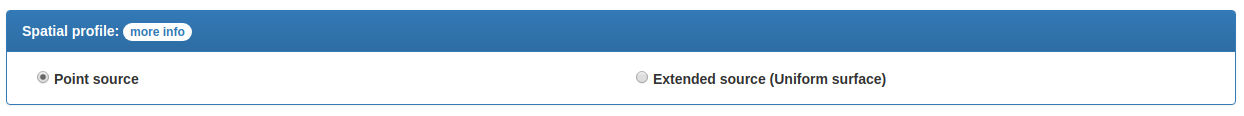
\includegraphics[scale=0.25]{figs/spatial-profile}
    \label{fig:spatial}
\end{figure}
\begin{figure}[h]
    \centering
    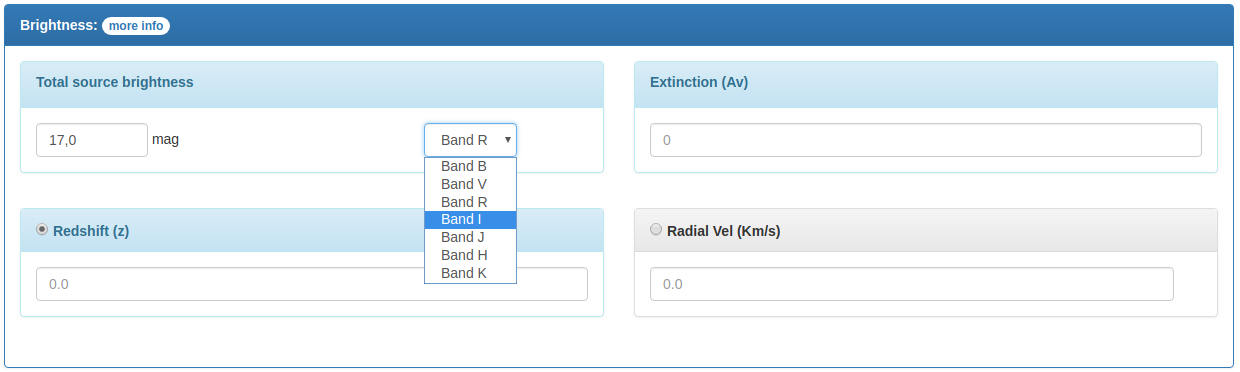
\includegraphics[scale=0.25]{figs/brightness}
    \label{fig:brightness}
\end{figure}
\begin{figure}[h]
    \centering
    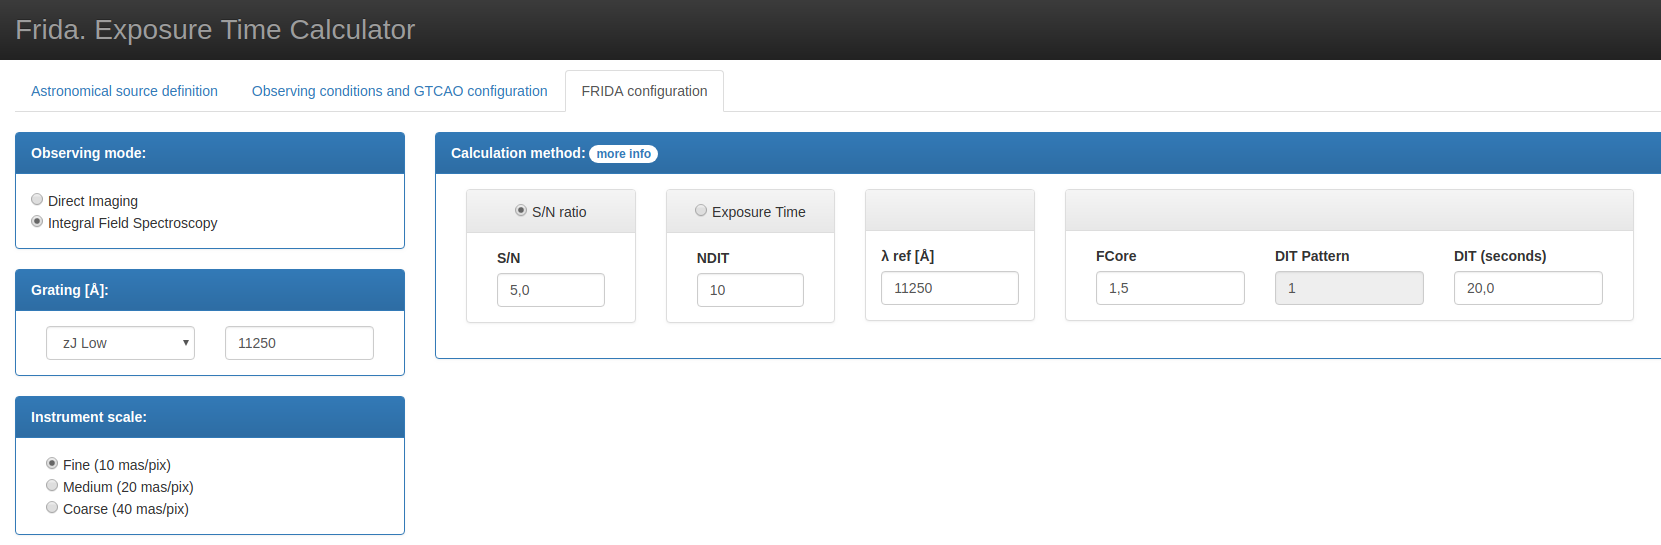
\includegraphics[scale=0.2]{figs/ifs-mode}
    \caption{Modo IFS}
    \label{fig:ifs-mode}
\end{figure}
\begin{figure}[h]
    \centering
    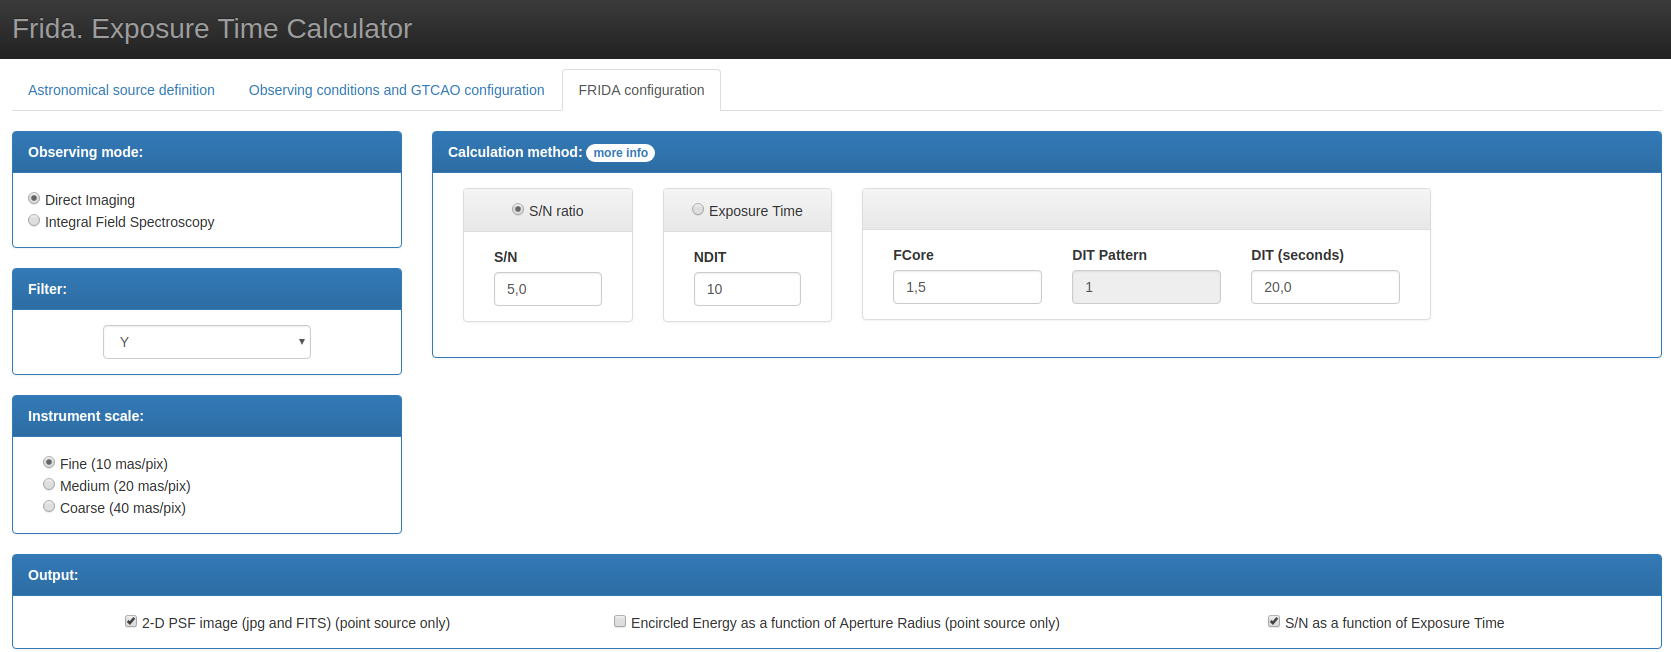
\includegraphics[scale=0.2]{figs/image-mode}
    \caption{Modo Imagen}
    \label{fig:image-mode}
\end{figure}



\end{document}
